\documentclass[../main/main.tex]{subfiles}

\newdate{date}{13}{11}{2019}


\begin{document}

\chapter{The role of dimension, symmetry and range of interactions in phase transitions}


\marginpar{ \textbf{Lecture 10.} \\  \displaydate{date}. \\ Compiled:  \today.}


Which is the role of the dimension in phase transition? Consider \emph{d}, the dimension of the system.
For the Ising model, we have seen that in \( d=1 \) there is no phase transition, while the Onsanger solution tell us that for \( d=2 \) there is a paramagnetic-ferromagnetic transition for \( T_c >0 \).
Therefore, the dimension seems a crucial parameter!
Since in general analytic solutions are not available, is there a simple argument to establish the existence of a phase transition?
In the case of a para-ferro transition, may we establish whether a phase with long range order exists and is stable within a range of \( T>0 \)?

\section{Energy-entropy argument}
We need an argument that can tell us which kind of system has a phase transition. The idea is to use the entropy energy argument. Indeed, our systems are ruled by a free energy and the previous states are found by making derivative. We have energy and entropy: low energy state can be stable with respect to thermal fluctuations, but the fluctuations will destroy the long range order. This idea can be generalized.

Let us consider: 
\begin{equation}
  \dd[]{F} = \underbrace{\dd[]{U}}_{\text{energy}}  - T \underbrace{ \dd[]{S}}_{\text{entropy}}
\end{equation}
We expect that:
\begin{itemize}
\item \( T \gg 1\): entropy should dominates.
\item \( T \ll 1 \): energy should dominates.
\end{itemize}

\noindent Question: there is a temperature different to zero in which this is compatible?

\subsection{\emph{1-dim} Ising}
Let us study the stability of the states with minimum energy to fluctuations for \( T \neq 0 \), for a system of size  \emph{N}.

We already know that, for \( T=0 \), two ground states exist, either all spins up or all spins down.
For instance, suppose that we have the ground state with all the spin up; the energy of the state is
\begin{equation}
   E_G = -JN
\end{equation}
and it is the same for the other configuration.

Now, let us consider \( T \neq 0 \), there could be a given number of elementary excitations of the kind spin up/down. What happens if we swap one or more spins?
These are defects with respect to the ground state and they are also called \emph{domain walls}.
This is in the one dimensional case, but is valid also in many dimensional. Therefore, which is the variation in energy \( \Delta E \) with respect to the ground state?
For each excitation there is an energy penalty \( \Delta E = 2J \), indeed, if we suppose that we have only one swap, we have 
\begin{equation*}
  E_G = -JN, \qquad E^* = -J(N-1) +J \qquad \Rightarrow \Delta E = 2J
\end{equation*}
For a finite concentration \emph{x} of domain walls, we can write \(   M = Nx \), giving
\begin{equation}
  \Delta E_M = 2MJ
\end{equation}

Now, let us compute the change in entropy.
The entropy of the ground state can be computed immediately: this is zero because it is the logarithm of the number of configurations, but in this case we have only one configuration, namely  \( S_G = \ln{1} =  0 \). Hence, the difference between the entropy of the ground state and the entropy of the new state is just the entropy of the new state.
Therefore, we want to estimate the entropy of the states with \emph{M} domain walls. 
The number of possible ways to insert \emph{M} domains in \emph{N} positions, namely the number of configurations, is
\begin{equation}
  \# = \begin{pmatrix}
  N \\
  M
  \end{pmatrix} = \begin{pmatrix}
  N \\
  xN
  \end{pmatrix}
\end{equation}
We have:
\begin{equation}
  S_M = k_B \log{\begin{pmatrix}
  N \\
  M
  \end{pmatrix}}
\end{equation}
the difference is
\begin{equation*}
  \Delta S = S_M -S_G = S_M = k_B \ln{\begin{pmatrix}
  N \\
  xN
  \end{pmatrix} }
\end{equation*}
Let us calulate
\begin{equation*}
\begin{split}
\Delta F  &= F_M - F_G = \Delta E - T \Delta S  \\
          &= 2 M J - k_B T \ln{\begin{pmatrix}
          N \\
          M
          \end{pmatrix} } \\
          & = 2xNJ - k_B T \ln{\begin{pmatrix}
          N \\
          xN
          \end{pmatrix} } \\
          & = N \qty{ 2xJ +k_B T \qty[x \ln{x} + (1-x)\ln{(1-x)}  ] }
\end{split}
\end{equation*}
where we have used the Stirling approximation
\begin{equation*}
 \ln{N!} = N \ln{N} - N   
\end{equation*}
Since the equilibrium states are obtained by the minimum of \emph{F}, we can minimize with respect to \emph{x}. We are interested in the free energy in the bulk, hence, firstly we normalize and then we derive for finding the minimum
\begin{equation}
  \Delta f_{b_N} = \frac{\Delta F_N}{N}, \qquad \pdv{\Delta f_b}{x} = 0
\end{equation}
this gives 
\begin{equation*}
\begin{split}
  \pdv{}{x} \qty{ 2xJ +k_B T \qty[x \ln{x} + (1-x)\ln{(1-x)}  ] } &=  2J + k_B T \qty[\ln{x} +1 -\ln{(1-x)} -1 ]\\
  & = 2J + k_B T \qty[\ln{x}- \ln{(1-x)}  ] = 0
\end{split}
\end{equation*}
hence,
\begin{equation*}
  \ln{\frac{x}{1-x}} = -\frac{2J}{k_B T} \quad \Rightarrow \frac{x}{1-x} = e^{-2J/k_BT}
\end{equation*}
and finally the results is
\begin{equation}
 x = \frac{1}{1+e^{2J/k_BT} }
 \label{eq:10_3}
\end{equation}
It means that  \( \forall T \neq 0 \) exist a finite concentration \emph{x} of domain walls. The ground state is unstable \( \forall T>0 \). Indeed, if you have a finite density of \emph{x}, no long range order exist for \( T>0 \).  From \eqref{eq:10_3}, we can see that as \( T \rightarrow 0 \),  we have \( x \rightarrow 0\) as expected.
Now, let us try to do the same for \emph{d} dimensions.

\subsection{\emph{d-dim} Ising}
What is a \emph{domain wall} in \emph{d} dimensions? The domain walls is an hypersurface of size \( L^{d-1} \)
\begin{equation}
  \Delta E \propto 2JL^{d-1}
\end{equation}
Computing the entropy it is a very difficult problem. Indeed, the entropy of a fluctuating hypersurface is difficult to estimate. 
For a single domain wall, we can say
\begin{equation}
  S \ge k_B \ln{L}
\end{equation}
where  \emph{L} is the number of ways to place a straight wall within a system of linear size \emph{L}.
The \( \Delta S \)  is just \emph{S}  because the entropy of the ground state is again zero.
\begin{remark}
If we underestimate \emph{S}, we obtain
\begin{equation}
  \Delta F = 2JL^{d-1}-k_B T \ln{L}
\end{equation}
it means that now energy can win if the temperature is different from zero. Therefore, for \( d=2 \),  or greater (\( d>1 \)), that long range order can survive  thermal fluctuations and the system could present an ordered phase!
\end{remark}

\subsubsection{Peierls argument}
The Peierls argument \cite{10_lesson_1} is a mathematically rigorous and intuitive method to show the presence of a non-vanishing spontaneous magnetization in some lattice models. This argument is typically explained for the \(d=2\) Ising model in a way which cannot be easily generalized to higher dimension.
The idea is trying to perturb the system using an external magnetic field as perturbation (it is very small \emph{h}). In that way, we are breaking explicitly the symmetry, but then, taking the limit \( h \rightarrow 0 \) and switching off the magnetic field, we see the stability.

 We know that for finite systems, from the \( \mathbb{Z}^2 \) symmetry, it follows
\begin{equation*}
  \expval{m}_N = 0
\end{equation*}
This is true for finite systems, however, in the thermodynamical limit \( N \rightarrow \infty  \), if \(d \ge 2\) the magnetization \( \expval{m}_{\infty } \) vanishes only in the high temperature paramagnetic phase. 
In the low temperature ferromagnetic phase, the value of \( \expval{m}_{\infty } \) is not well defined and depends on how the thermodynamical limit is performed. In this case the \( \mathbb{Z}^2\) symmetry  is said to be spontaneously broken.

The breaking of a symmetry can be thought as a form of thermodynamical instability: the particular value acquired by \( \expval{m}_{\infty } \) in the ferromagnetic phase is determined by small perturbations.

A conventional way to uniquely define \( \expval{m}_{\infty } \) in the broken phase (where it is called spontaneous magnetization) is to use an infinitesimal magnetic field:
\begin{equation}
  \expval{m}_{\infty } = \lim_{h \rightarrow 0^+} \lim_{N \rightarrow \infty } \expval{m}_N^{(h)}
\end{equation}
where it is crucial to perform the thermodynamical limit before switching off the magnetic field \( h \rightarrow 0^+ \). The instability manifests itself in that using \( h \rightarrow 0^- \)  would change the sign of \( \expval{m}_{\infty } \).

A different approach to expose the instability is the use of appropriate boundary conditions:
we can for example, if we want \( \expval{m}_ \infty  > 0\), impose in all the sites \(i\) on the lattice boundary (\( i \in \partial{\Omega }  \)) the condition
\( S_i = +1 \),  as in Figure \ref{fig:10_1}.

\begin{figure}[h!]
\centering
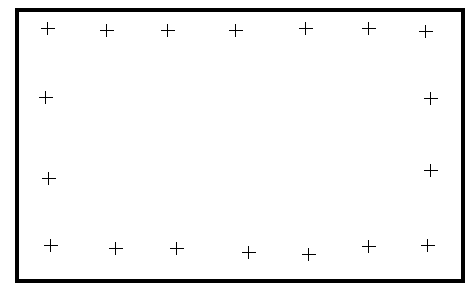
\includegraphics[width=0.5\textwidth]{../lessons/10_image/1.pdf}
\caption{\label{fig:10_1} System with boundary condition with all the spins in the surface up.}
\end{figure}

In the paramagnetic phase the effect of boundary conditions does not survive the thermodynamical limit, while in the ferromagnetic phase their effect is analogous to that of the infinitesimal magnetic field.
%\begin{remark}
 %It is equivalent, because on the border we have a very high field, but it is at the border, so it do not really count for the surface internal. This is a very smart way to do this perturbation of the surface. This particular configuration with all the spin up will give us a particular shape. We can do this also in higher dimensional and we can also estimate the temperature.
%\end{remark}

This is the boundary condition chosen by Pierls to establish the existence of a \( T_c \neq 0 \) for the \(d=2\) Ising model.
Let us gives just a qualitative presentation  of the (rigorous) result. 

Let \( N_+,N_- \) be the number of spin up and down respectively. Clearly,
\begin{equation*}
  N=N_+ + N_-  
\end{equation*}
On a finite lattice the mean value of the magnetization can be written in the form 
\begin{equation*}
  \expval{m}_N = \frac{\expval{N_+} - \expval{N_-}  }{N} = 1 - 2 \frac{\expval{N_-} }{N}
\end{equation*}
In order to show that \( \expval{m}_ \infty >0  \) (remember that we are considering boundary conditions with spin up at \( \partial{\Omega }  \)), it is sufficient to show that for every \(N\) we have 
\begin{equation}
  \frac{\expval{N_-} }{N}  < \frac{1}{2}- \varepsilon
  \label{eq:10_1}
\end{equation}
with \( \varepsilon >0 \) and \(N\)-independent.
Indeed, if \eqref{eq:10_1} holds
\begin{equation}
  \expval{m}_N \ge 2 \varepsilon \quad \forall N
\end{equation}
The Peierls argument is a simple geometrical construction that can be used to prove this
bound.
The outcome of the Peierls argument for the model in \(d\) dimensions is an estimate of the form
\begin{equation}
  \frac{\expval{N_-} }{N} \le f_D (x)
\end{equation}
where \(x\) is defined by 
\begin{equation}
  x = 9 e^{-4J \beta } 
\end{equation}
and \( f_D \) is a continuous function of \( x \) (independent on \emph{N}) and such that 
\begin{equation*}
\lim_{x \rightarrow 0} f_D (x) = 0    
\end{equation*}
In particular, for small enough \emph{T} we have the bound
\begin{equation*}
  \frac{\expval{N_-} }{N} < \frac{1}{2} - \varepsilon
\end{equation*}
which ensures that \(\expval{m}_\infty \ge 2\varepsilon  \) and the \(\mathbb{Z}^2\) symmetry is spontaneously broken.
More precisely, for \(d=2\), one has
\begin{equation}
    \frac{\expval{N_-} }{N} \le \frac{x^2}{36} \frac{2-x}{(1-x)^2}
\end{equation}
where \(   x = 9 e^{-4J \beta } < 1 \).

\begin{remark}
Note that above bound gives also a lower bound on the critical temperature
\begin{equation*}
    \frac{\expval{N_-} }{N} \le \frac{x^2}{36} \frac{2-x}{(1-x)^2} < \frac{1}{2} - \varepsilon
\end{equation*}
As long as \(   \frac{\expval{N_-} }{N}  < \frac{1}{2} - \varepsilon  \), the system is in the ferromagnetic phase. The critical value \( x_c \equiv x (\beta _c) \) must be outside the interval \( [0,x_{1/2}] \) where \( x_{1/2} \)   is the smallest positive solution of the equation
\begin{equation*}
  \frac{x^2}{36} \frac{2-x}{(1-x)^2} = \frac{1}{2}
\end{equation*}
From the solution \( x_{1/2} \) and the condition \( x_c > x_{1/2} \), one has
\begin{equation*}
  J \beta _c \le J \beta_{1/2}
\end{equation*}
where \( J \beta _{1/2} = \frac{1}{4} \log{9/x_{1/2}}  \). 
Hence, \( T_c > T_{1/2} \).
\end{remark}

\begin{exercise}{}{}
The following equation gives \( x_{1/2} \):
\begin{equation*}
  x^3 + 16x^2 - 36 x + 18 = 0
\end{equation*}
 Find \( T_{1/2} \).
\begin{solution}
This equation has three real solutions:
\begin{equation*}
    x_1 =-18.05, \quad x_2=0.79, \quad x_3=1.26
\end{equation*}
The smallest positive solutions is \( x_{1/2} \equiv x_2 \), hence 
\begin{equation*}
\frac{J}{k_B T_{1/2} } = \frac{1}{4} \log{9/x_{1/2}} \quad \Rightarrow 
T_{1/2} = \frac{4J}{k_B \log{9/x_{1/2}}}
\end{equation*}
\end{solution}
\end{exercise}


\clearpage
\section{Role of the symmetry}
Interacting systems can be classified with respect to their \emph{global symmetry group}. Let us illustrate some examples.
\begin{example}{Ising model}{}
  \begin{equation}
    \mathcal{H}_{\text{Ising}} = - \sum_{i<j}^{} J_{ij} \sigma _i \sigma _j
  \end{equation}
  where \( \sigma _i \in \{ -1,1 \}   \). The symmetry gropu of this Hamiltonian is \( \mathbb{Z}^2 \), which has two elements \( \{ \mathbb{1}, \mu  \}   \). We have
  \begin{equation}
    \mathbb{1}: \text{ identity}, \quad \mu \sigma _i = - \sigma _i, \quad \mu ^2 = \mathbb{1}
  \end{equation}
\end{example}
\begin{example}{Potts model}{}
  \begin{equation}
    \mathcal{H}_{q- \text{Potts}} = - \sum_{i<j}^{} J_{ij} \delta _{\sigma _i, \sigma _j}
  \end{equation}
  where \( \sigma _i \in [1,2,3,\dots,q] \). \( \mathcal{H}_{q- \text{Potts}} \)  is invariant under the permutation group of the sequence \( \{ 1,2,3,\dots,q \}   \). There are \( q! \) elemtns, for example \( \{ 2,1,3,\dots,q \}   \). The symmetry group is denoted by \( S_q \).
\end{example}
\begin{remark}
The difference between a \( \mathbb{Z}_q \) and \( S_q \) symmetry is that an Hamiltonian has symmetry \( \mathbb{Z}_q \) if it is invariant with respect to \emph{cyclic permutations}
\begin{equation}
  \mu = \begin{pmatrix}
    1 & 2 & \dots & q-1 & q \\
    2 & 3 & \dots & q & 1
  \end{pmatrix}
\end{equation}
and its powers \( \mu ^l \) with \( l=0, \dots, q-1 \). Both models satisfy a \emph{discrete global symmetry}.
\end{remark}
Now, we jump into the case in which we consider \emph{continuous} symmetries.

\section{XY model}
This is a spin model that is invariant with respect to the continuous global symmetry
\( \theta _i \rightarrow \theta _i + \alpha  \).
Indeed the Hamiltonian of this model is
\begin{equation}
  \mathcal{H}_{XY} = - \sum_{i<j}^{} J_{ij} \va{S}_i \vdot \va{S}_j
\end{equation}
where \(\va{S}_i  \) is a \( 2D \) spin vector
\begin{equation}
  \va{S}_i = (S_{x_i}, S_{y_i})
\end{equation}
that can assume values on the unit circle ( \(  \abs{\va{S}_i} =1 \)).

Suppose that you have spins that are sitting in hyper dimensional. Rotate along a circle this spins. They can assume all the value as in Figure \ref{fig:10_2}.

\begin{figure}[h!]
\centering
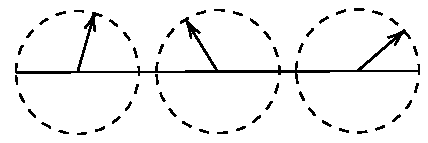
\includegraphics[width=0.5\textwidth]{../lessons/10_image/2.pdf}
\caption{\label{fig:10_2} }
\end{figure}
The simplest way to parametrize the Hamiltonian is by the angle.
Denoting by \( \theta _i \) the direction angle of spins \( \va{S}_i \), the \( \mathcal{H}_{XY} \) can be written as
\begin{equation}
  \mathcal{H}_{XY} = - \sum_{i<j}^{} J_{ij} \cos(\theta _i - \theta _j)
\end{equation}
with \( \theta _i \in [0,2 \pi ] \).
\begin{remark}
The interaction term \( \cos(\theta _i - \theta _j)  \) can be written also as
\begin{equation}
  \frac{1}{2} \qty(Z_i^* Z_j + Z_i Z_j^*)
\end{equation}
where \(   Z_j = \exp (i \theta _j) \).
\end{remark}
The model is invariant under the global transformation
\begin{equation}
  Z_i \rightarrow e^{i \alpha } Z_i
\end{equation}
The phase  \( \exp (i \alpha )  \) form a group under multiplication known as \( U(1) \) that is equivalent to \( O(2) \). Indeed the interaction term can be written also as
\begin{equation}
  \vu{\Omega }_i \vdot \vu{\Omega }_j
\end{equation}
where \( \vu{\Omega }_i = ( \cos \theta _i, \sin \theta _i) \).
\begin{remark}
In \emph{n}-dimensions \( \vu{\Omega } \) has \emph{n} components  \( \vu{\Omega } = \{ \Omega ^1, \Omega ^2, \dots, \Omega ^n \}   \)  and the corresponding Hamiltonian
\begin{equation}
  \mathcal{H} = - \sum_{i>j}^{} J_{ij} \vu{\Omega }_i \vdot  \vu{\Omega }_j
\end{equation}
It is symmetric with respect to the global symmetry group \( O(n) \).
\end{remark}
 Which are the domain walls for continuous symmetries? Which are the implications for the stability of the ordered phase?



\section{Continuous symmetries and phase transitions}
The questions is: when it is not continuous which is the boundary?
When the symmetry is continuous the domain walls interpolate smootly between two ordered regions (see Figure \ref{fig:10_3}).

\begin{figure}[h!]
\centering
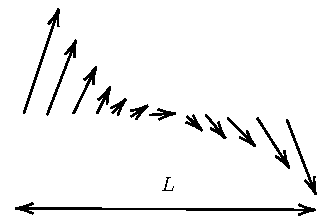
\includegraphics[width=0.4\textwidth]{../lessons/10_image/3.pdf}
\caption{\label{fig:10_3} }
\end{figure}
The energy term that in Ising is proportional to \( 2JL^{D-1} \) how does it change here?
Suppose that the variation of the direction between two neirest neighbours sites is very small, i.e. \( (\theta _i - \theta _j) \ll 1 \) for \( i,j \) neirest neighbours.
 Now we can diluite the energy, in other words weak the energy term.

Let us do a Taylor expainding of the interaction term
\begin{equation}
  \cos (\theta _i - \theta _j) \simeq 1 - \frac{1}{2} (\theta _i - \theta _j)^2 \Rightarrow \sum_{\expval{ij} }^{}  \qty(1 - \frac{1}{2} (\theta _i - \theta _j)^2)
  \label{eq:10_2}
\end{equation}
The Hamiltonian can be written as
\begin{equation}
  \mathcal{H} \simeq - J \sum_{\expval{ij} }^{} \qty(1- \frac{1}{2}(\theta _i - \theta _j)^2)
\end{equation}
The \eqref{eq:10_2} corresponds to the discrete differential operator where
\( \theta _i - \theta _j = \partial_x{\theta }  \),
therefore
\begin{equation}
  \mathcal{H} = E_0 + \underbrace{\frac{J}{2} \int_{}^{} \dd[]{\va{r}} \qty(\grad \theta )^2 }_{E \equiv \text{Stifness energy}}
\end{equation}
where \( E_0 = 2JN \) is the energy corresponding to the case in which all the spins are oriented along a given direction.

\begin{definition}{Stifness energy}{}
  The Stifness energy is defined as
  \begin{equation}
    E = \frac{J}{2} \int_{}^{} \dd[]{\va{r}} \qty(\grad \theta )^2
  \end{equation}
where \( \theta (\va{r})  \) is the angle of a local rotation around an axis and \emph{J} is the \emph{spin rigidity}. For an ordered phase \( \theta (\va{r}) = \theta _0 \).
\end{definition}
Let us now imagine a domain wall where \(\theta (\va{r})  \)  rotates by \( 2 \pi  \) (or \( 2 \pi m \)) by using the entire length of the system (see again Figure \ref{fig:10_3}):
\begin{equation}
  \theta (\va{r}) = \frac{2 \pi n x}{L}
\end{equation}
where \emph{n} is the total number of \( 2 \pi  \) turn of \( \theta  \) in \emph{L}. Note that there is no variation along the other \( D-1 \) dimensions, therefore we just doing over one dimension.

 Consider only the term called \emph{E}
 \begin{equation}
   E = \frac{J}{2} L^{D-1} \int_{0}^{L} \dd[]{x} \qty(\dv{}{x} \qty(\frac{2 \pi n x}{L})  )^2 = \frac{J}{2} L^{D-1} \int_{0}^{L} \dd[]{x} \qty(\frac{2 \pi n}{L})^2 \approx 2 \pi ^2 n^2 J L^{D-2}
 \end{equation}
\begin{remark}
Unlike the Ising model where \( E \sim L^{D-1} \), here \( E \sim L^{D-2} \)!

If \( S \ge k_B \ln{L}  \) for a single domain wall, \emph{S} should dominate if \( D \le 2 \), the ordered phase is always unstable and no phase transition is expected for \( T \neq 0 \)!
\end{remark}

\begin{definition}{Lower critical dimension}
  The Lower Critical dimension \( D_c \) is the dimension at which (and below which) the system does not display a ordered phase (there is no long range order).
  In other words if \( D \le D_c \), we have \( T_c = 0 \).
\end{definition}
\begin{theorem}{Mermin-Wagner}{}
  For continuous global symmetries the \( D_c =2 \).
\end{theorem}

 From what we have dound before we can say that
\begin{itemize}
\item Discrete global symmetries: \( D_c =1 \).
\item Continuous global symmetries: \( D_c =2 \).
\end{itemize}

\begin{remark}
The \emph{XY} model in \( D=2 \) is rather special. Although it dos not display an ordered phase, there exist at \( T \neq 0 \) a special phase transition known as the \emph{Kosterlitz-thouless transition}. This transition dows not imply the spontaneous breaking of the \( O(2) \) symmetry! There is no long range order for \( T<T_{KT} \) (statistic of vortices, topological defects in \( D=2 \)).
\end{remark}


\section{Role of the interaction range}
So far we have considered models where the interactions were short range. How things change if long range are considered instead? How does the symmetry broken depends on the range of interactions? One can show, for example, that if
\begin{equation}
  J_{ij} = \frac{J}{\abs{\va{r}_i - \va{r}_j}^\alpha  }
\end{equation}
with \( 1 \le \alpha \le 2 \), phase with long range order is stable for \( 0 < T < T_c \) also for \( D=1 \)!   So we have a long range order with \( T_c \neq 0 \), even for \( D=1 \)!

\begin{remark}
If \( \alpha > 2 + \varepsilon  \) we get back the physics found for short range interactions. If \( \alpha <1 \) the thermodynamic limit does not exist.
\end{remark}
A limiting case of long range interaction is the infinite range case where all the spins interact one to another with the same intensity indipendently on their distance. No metric is involed (instead of previously where the definition of \emph{J} of before is a metric.). It can be solve exactly and later we will seen why.


\section{Ising model with infinite range}

The Hamiltonian is the following:
\begin{equation}
  -\mathcal{H}_N (\{ S \} ) = \frac{J_0}{2} \sum_{i,j}^{N} S_i S_j + H \sum_{i}^{}  S_i
\end{equation}
with \( S_i \in [-1,+1] \). The problem is the double sum over \emph{i,j}, indeed
\begin{equation}
  \sum_{i,j}^{} S_i S_j \propto O(N^2)
\end{equation}
and the thermodynamic limit is ill-defined. To circumvent this problem \emph{Kac}  suggested to consider a strength
\begin{equation}
  J_0 = \frac{J}{N}
\end{equation}
this is called the \emph{kac} approximation
\begin{equation}
  -\mathcal{H}_N (\{ S \} ) = \frac{J}{2N} \sum_{i,j}^{N} S_i S_j + H \sum_{i}^{}  S_i
\end{equation}
with this choice we recover \( E \sim O(N) \).  In this Hamiltonian since you have no metric you have no dimension.





\end{document}
